\documentclass[9pt]{beamer}
\usepackage[sfdefault]{roboto}
\usepackage[utf8]{inputenc}
\usepackage[T1]{fontenc}
\usepackage{styles/fluxmacros}
\usefolder{styles}
\usetheme[style=asphalt]{flux}
\usepackage{booktabs}
\usepackage{colortbl}
\usepackage{ragged2e}
\usepackage{schemabloc}
%~~~~~~~~~~~~~~~~~~~~~~~~~~~~~~~~~~~~~~~~~~~~~~~~~~~~~~~~~~~~~~~~~~~~~~~~~~~~~~

%~~~~~~~~~~~~~~~~~~~~~~~~~~~~~~~~~~~~~~~~~~~~~~~~~~~~~~~~~~~~~~~~~~~~~~~~~~~~~~
% Informations
\title{Modeling and Simulation with SDEs}
\subtitle{a minicourse}
\author{SDIV}
\institute{CONACYT-UNIVERSIDAD DE SONORA, Guanajuato, Gto.}
\date{\today}
\titlegraphic{assets/overleaf.png}
%~~~~~~~~~~~~~~~~~~~~~~~~~~~~~~~~~~~~~~~~~~~~~~~~~~~~~~~~~~~~~~~~~~~~~~~~~~~~~~

\begin{document}

% Generate title page
\titlepage

\begin{frame}
 \frametitle{Table of contents}
 \tableofcontents
\end{frame}

\section{Presentation}

\subsection{introduction}

\begin{frame}{Flux}{introduction}
	\justifying
 Flux is a modern style beamer presentation. It is provided as a work in progress version and may suffer from inconsistencies. Sources and complementary information are available at\\[0.3cm]
 	\centering\textbf{github.com/pvanberg/flux-beamer}
\end{frame}

\def\beamer@mytheme@style{green}
\begin{frame}[fragile]{Flux}{colors}
	\centering
	Flux provides five differents color palettes.\\
	\verb+\usetheme[style=asphalt]{flux}+\\[0.8cm]
	\newcommand{\colorRow}[1]{
	\begin{tabular}{p{4cm}cccc}
	#1 & \cellcolor{primary}\hspace*{1cm} &\cellcolor{primaryLight}\hspace*{1cm}&\cellcolor{secondary}\hspace*{1cm}&\cellcolor{tertiary}\hspace*{1cm}\\
 	\end{tabular}
 	}
 	\colorRow{Asphalt}\\[0.3cm]
	\definecolor{primaryLight}{HTML}{3a99d9}
	\definecolor{primary}{HTML}{2e81b7}
	\definecolor{secondary}{HTML}{2e81b7}
	\definecolor{tertiary}{HTML}{e76d55}
 	\colorRow{Blue}\\[0.3cm]
    \definecolor{primaryLight}{HTML}{77933c}
    \definecolor{primary}{HTML}{4f622a}
    \definecolor{secondary}{HTML}{884F4D}
    \definecolor{tertiary}{HTML}{2B3234}
 	\colorRow{Green}\\[0.3cm]
 	\definecolor{primaryLight}{HTML}{C0392B}
    \definecolor{primary}{HTML}{96281B}
    \definecolor{secondary}{HTML}{347986}
    \definecolor{tertiary}{HTML}{56423e}
 	\colorRow{Red}\\[0.3cm]
 	\definecolor{primaryLight}{HTML}{616161}
	\definecolor{primary}{HTML}{424242}
	\definecolor{secondary}{HTML}{518071}
	\definecolor{tertiary}{HTML}{8b7687}
 	\colorRow{Gray}\\[0.3cm]
\end{frame}

\subsection{fonts}

\begin{frame}[fragile]{Flux}{fonts}
 Flux recommends the use of Roboto or Overpass font and a font size of 9pt.\\[0.2cm]
 \begin{center}
 	\verb+\documentclass[9pt]{beamer}+\\
	\verb+\usepackage[sfdefault]{roboto}+
 \end{center}
 
  Flux also implements default typographies.

	\begin{itemize}
		\item Regular
		\item \alert{Alert}
		\item \example{Example}
		\item \textit{Italic}
		\item \textbf{Bold}
	\end{itemize}
	
\end{frame}

\subsection{footnotes}

\begin{frame}{Flux}{footnotes}
		Flux also includes custom footnote integration. For instance, this \textbf{element}\footnote{Footnotes are notes placed at the bottom of a page. They cite references or comment on a designated part of the text above it. For example, say you want to add an interesting comment to a sentence you have written, but the comment is not directly related to the argument of your paragraph. } and this \textbf{element}\footnote{Footnotes are not just for interesting comments, however. Sometimes they simply refer to relevant sources -- they let your reader know where certain material came from, or where they can look for other sources on the subject.} provide a footnote.
\end{frame}

\section{Collections}
\subsection{lists}

\begin{frame}{Flux}{lists}
   \begin{columns}[T,onlytextwidth]
    \column{0.33\textwidth}
      \textbf{Items}
      \begin{itemize}
        \item Cats \item Dogs \item Birds
      \end{itemize}

    \column{0.33\textwidth}
      \textbf{Enumerations}
      \begin{enumerate}
        \item First \item Second \item Last
      \end{enumerate}

    \column{0.33\textwidth}
      \textbf{Descriptions}
      \begin{description}
        \item[Apples] Yes \item[Oranges] No \item[Grappes] No
      \end{description}
\end{columns}
\let\thefootnote\relax\footnote{Note the following demo slides are directly taken from metropolis theme. Copyright 2014 Matthias Vogelgesang.\\
Give a look at https://github.com/matze/mtheme/tree/master/demo}
\end{frame}

\subsection{tables}

\begin{frame}{Flux}{tables}
  \begin{table}
    \caption{Largest cities in the world (source: Wikipedia)}
    \begin{tabular}{@{} lr @{}}
      \toprule
      City & Population\\
      \midrule
      Mexico City & 20,116,842\\
      Shanghai & 19,210,000\\
      Peking & 15,796,450\\
      Istanbul & 14,160,467\\
      \bottomrule
    \end{tabular}
    \hspace*{1cm}
        \setlength\extrarowheight{3pt}
    \begin{tabular}{|lr|}
      \hline
      \rowcolor{primaryLight}\color{background}City & \color{background}Population\\
      \hline
      Mexico City & 20,116,842\\
      Shanghai & 19,210,000\\
      Peking & 15,796,450\\
      Istanbul & 14,160,467\\
      \hline
    \end{tabular}
\end{table}
\end{frame}

\subsection{blocs}

\begin{frame}[fragile]{Flux}{blocks}
  		Flux theme comes with three pre-defined block style collections.\\
  		Native style (default) available as \verb+\setblockstyle{native}+\\[0.5cm]
  
   \setblockstyle{native} % Default behavior, optional line.
   \centering
	\begin{minipage}[b]{0.5\textwidth}

	  \begin{block}{Default}
        Block content.
      \end{block}

      \begin{alertblock}{Alert}
        Block content.
      \end{alertblock}

      \begin{exampleblock}{Example}
        Block content.
      \end{exampleblock}      
      
	\end{minipage}
	
\end{frame}

\begin{frame}[fragile]{Flux}{blocks}
  		Flux theme comes with three pre-defined block style collections.\\
  		NoBackground style available as \verb+\setblockstyle{nobackground}+\\[0.5cm]
  
   \setblockstyle{nobackground}
   \centering
	\begin{minipage}[b]{0.5\textwidth}

	  \begin{block}{Default}
        Block content.
      \end{block}

      \begin{alertblock}{Alert}
        Block content.
      \end{alertblock}

      \begin{exampleblock}{Example}
        Block content.
      \end{exampleblock}       
      
	\end{minipage}
	
\end{frame}

\begin{frame}[fragile]{Flux}{blocks}
  		Flux theme comes with three pre-defined block style collections.\\
  		Metropolis style available as \verb+\setblockstyle{metropolis}+\\[0.5cm]
  
   \setblockstyle{metropolis}
   \centering
	\begin{minipage}[b]{0.5\textwidth}

	  \begin{block}{Default}
        Block content.
      \end{block}

      \begin{alertblock}{Alert}
        Block content.
      \end{alertblock}

      \begin{exampleblock}{Example}
        Block content.
      \end{exampleblock}      
      
	\end{minipage}
	
\end{frame}

\begin{frame}{Flux}{diagrams}
\centering
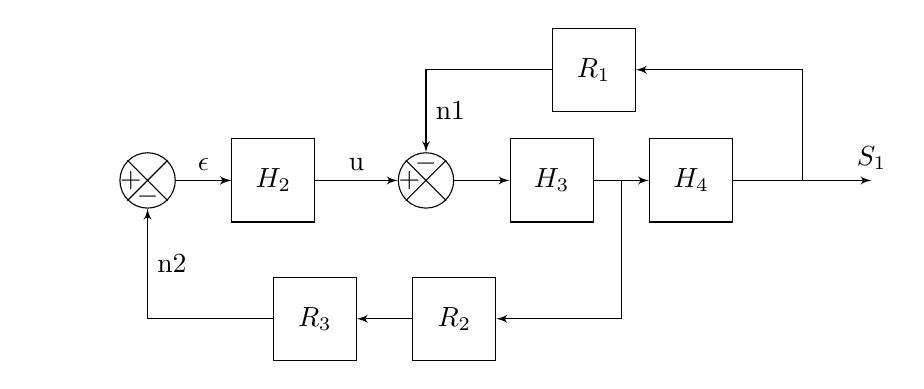
\begin{tikzpicture}
    \sbEntree{E}
    \sbComp{a}{E}
    \sbBlocL{c}{$H_2$}{a}
            \sbRelier[$\epsilon$]{a}{c}
    \sbComph{d}{c}
            \sbRelier[u]{c}{d}
    \sbBlocL{e}{$H_3$}{d}
    \sbBlocL{f}{$H_4$}{e}
    \sbSortie[5]{S1}{f}
            \sbRelier{f}{S1}
            \sbNomLien[0.8]{S1}{$S_1$}
    \sbDecaleNoeudy[-4]{f}{u}
    \sbDecaleNoeudy{e}{v}
    \sbBlocr{r1}{$R_1$}{u}
    \sbBlocr{r2}{$R_2$}{v}
    \sbBlocrL{r3}{$R_3$}{r2}
    \sbRelieryx{f-S1}{r1}
    \sbRelierxy[n1]{r1}{d}
    \sbRelieryx{e-f}{r2}
    \sbRelierxy[n2]{r3}{a}
\end{tikzpicture}\\[0.4cm]
Bloc diagram example from \textbf{texample.net}
\end{frame}

\begin{frame}{Flux}{plots}
	\begin{minipage}{0.56\textwidth}
		\begin{figure}
			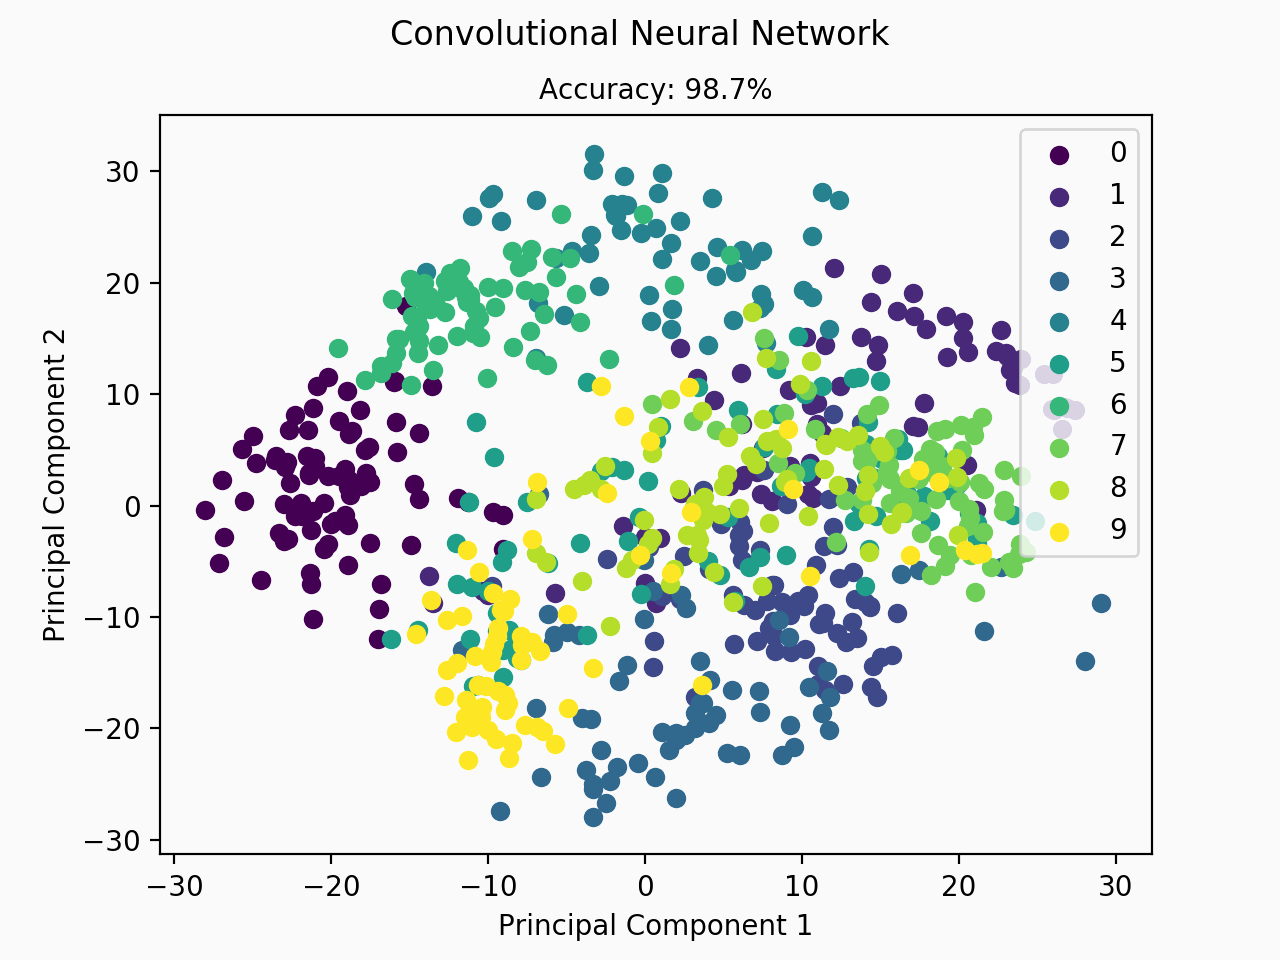
\includegraphics[width=\textwidth]{assets/plot.png}
		\end{figure}
	\end{minipage}
	\hfill
	\begin{minipage}{0.38\textwidth}
		\begin{block}{Binary Softmax classifier}
			\centering
			$\sigma(\sum_i w_ix_i + b)$
		\end{block}
		\begin{exampleblock}{Loss function}
			\centering\vspace*{0.1cm}
			$L_i = -log(\frac{e^{f_{y_i}}}{\sum_j e^{f_j}})$\\[0.1cm]
			cross entropy
		\end{exampleblock}
	\end{minipage}
\end{frame}

% The [plain] causes the headlines, footlines, and sidebars 
% to be suppressed. Useful for showing large pictures
\begin{frame}[plain]
	\begin{center}
	  This is a plain frame.\\
	  Use it to display full page images.
	  \end{center}
\end{frame}

\begin{frame}[allowframebreaks]{References}

  \nocite{*}
  \bibliography{demo}
  \bibliographystyle{abbrv}

\end{frame}

\section{Next section}
\subsection{subsection 1}
\subsection{subsection 2}
\subsection{subsection 3}
\section{One more section}
\subsection{subsection 1}
\subsection{subsection 2}
\subsection{subsection 3}

\begin{frame}
 \centering
 \frametitle{Flux}
 \framesubtitle{license}
 Flux is licensed under GNU General Public License v3.\\[0.3cm]
 	\centering\textbf{http://www.gnu.org/licenses}\\[0.3cm]
Inspired by \textbf{Metropolis} theme from Matthias Vogelgesang.\\
https://github.com/matze/mtheme 
 
\end{frame}

\end{document}